Grover algorithm and some nasty NMR computing at the end!

\begin{parts}
	\part Universal single qubit gates are the set of gates that form the basis of constructing a general qubit operation to an arbitrary accuracy, in this case $\mathrm{H}$ and $\mathrm{T}$ gates may replicate other single qubit operations to $F ~ 1$.
	
	X:
	\begin{figure}[H]
		\centering
		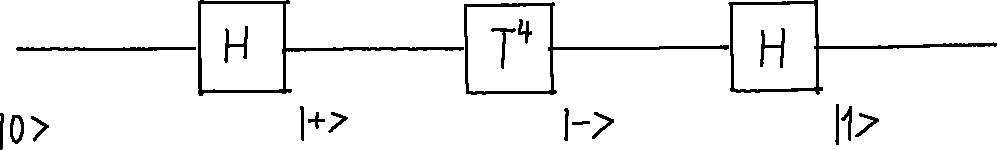
\includegraphics[width=.6\linewidth]{q6-x}
	\end{figure}
	
	Y:
	\begin{figure}[H]
		\centering
		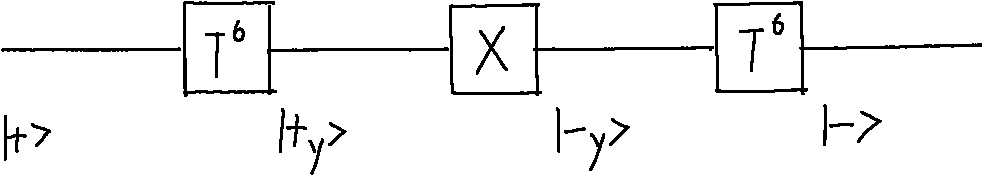
\includegraphics[width=.6\linewidth]{q6-y}
	\end{figure}
	
	Z:
	\begin{figure}[H]
		\centering
		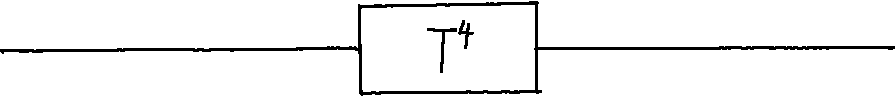
\includegraphics[width=.6\linewidth]{q6-z}
	\end{figure}
	
	\part Grover for $n=2$: $f:\cbracket{0,\, 1}^2 \rightarrow \cbracket{0,\, 1}$ only one $x$ gives $f(x) = 1$.
	\begin{figure}[H]
		\centering
		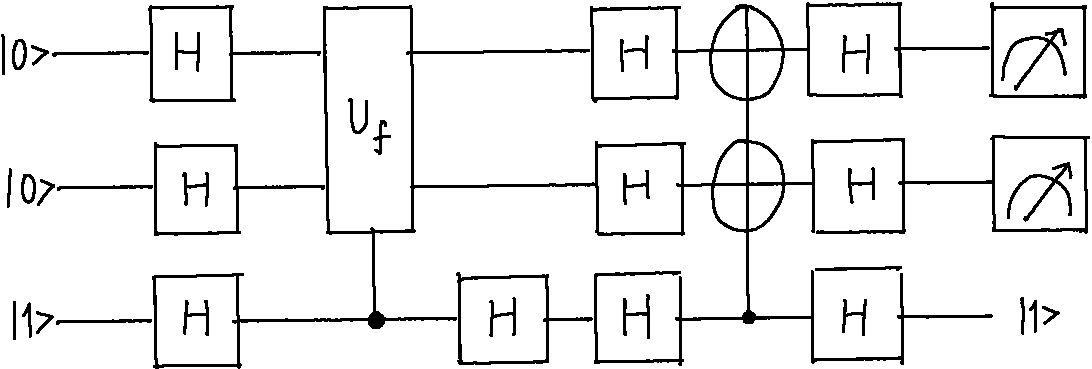
\includegraphics[width=.8\linewidth]{q6-grover}
	\end{figure}
	
	Note that the operation $\ket{x}\ket{y} \rightarrow \ket{x}\ket{y \oplus f(x)}$ with $x\equiv$ the input, $y\equiv$ the ancilla becomes $\ket{x}(\ket{0} - \ket{1}) \rightarrow \ket{x}(\ket{0 \oplus f(x)} - \ket{1 \oplus f(x)}) = (-1)^{f(x)} \ket{x}(\ket{0} - \ket{1})$ ignoring normalisation factor.
	
	Due to the linearity of Hilbert space, the phase $(-1)^{f(x)}$ may be thought of as being applied onto the superposition of inputs while leaving the ancilla unchanged, hence we may largely ignore ancilla in this algorithm for simplicity.
	
	A promise about $f$ is a specific fact that we know about $f$, without knowing the function itself.
	In Grover, the promise is that only one of the inputs returns $f(x) = 1$.
	
	We may then write $f_{jk}$ as the satisfying input being $\ket{jk}$.
	\begin{figure}
		\centering
		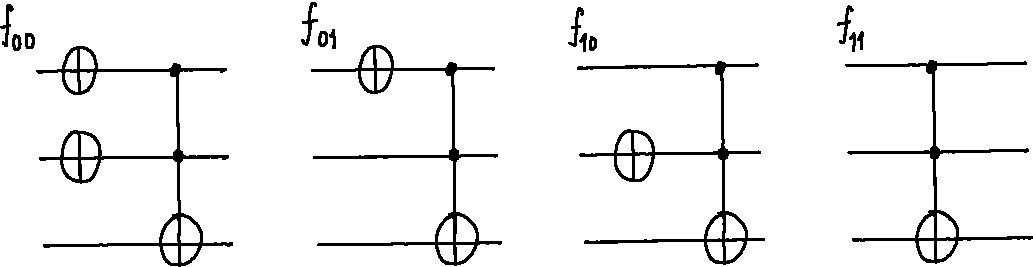
\includegraphics[width=.8\linewidth]{q6-fjk}
	\end{figure}
	
	After the oracle, we have states (in subspace of input qubits):
	\begin{align*}
		\ket{x} &= \ket{00} + \ket{01} - \ket{10} + \ket{11} \\
		&= \begin{pmatrix}
			1 \\ 1 \\ -1 \\ 1
		\end{pmatrix}
	\end{align*}
	
	We then have propagator:
	\begin{align*}
		\mathrm{H}^{\otimes 2} \cdot \mathtt{TOFFOLI} \cdot \mathrm{H}^{\otimes 2} &=
		\begin{pmatrix}
			1 & 1 & 1 & 1 \\
			1 & -1 & 1 & -1 \\
			1 & 1 & -1 & -1 \\
			1 & -1 & -1 & 1
		\end{pmatrix}
		\begin{pmatrix}
			1 & & & \\
			& 1 & & \\
			& & 1 & \\
			& & & -1
		\end{pmatrix}
		\begin{pmatrix}
			1 & 1 & 1 & 1 \\
			1 & -1 & 1 & -1 \\
			1 & 1 & -1 & -1 \\
			1 & -1 & -1 & 1
		\end{pmatrix} \\
		&= \begin{pmatrix}
			1 & 1 & 1 & 1 \\
			1 & -1 & 1 & -1 \\
			1 & 1 & -1 & -1 \\
			1 & -1 & -1 & 1
		\end{pmatrix}
		\begin{pmatrix}
			1 & 1 & 1 & 1 \\
			1 & -1 & 1 & -1 \\
			1 & 1 & -1 & -1 \\
			-1 & 1 & 1 & -1
		\end{pmatrix} \\
		&= \frac{1}{2}
		\begin{pmatrix}
			1 & 1 & 1 & -1 \\
			1 & 1 & -1 & 1 \\
			1 & -1 & 1 & 1 \\
			-1 & 1 & 1 & 1
		\end{pmatrix}
	\end{align*}
	
	Acting this on $\ket{x}$:
	\begin{align*}
		\begin{pmatrix}
			1 & 1 & 1 & -1 \\
			1 & 1 & -1 & 1 \\
			1 & -1 & 1 & 1 \\
			-1 & 1 & 1 & 1
		\end{pmatrix}
		\begin{pmatrix}
			1 \\ 1 \\ -1 \\ 1
		\end{pmatrix}
		&= \begin{pmatrix}
			0 \\ 4 \\ 0 \\ 0
		\end{pmatrix} \\
		&\propto \ket{01}
	\end{align*}
	
	Hence we obtain a unique output here, though a further $\mathtt{NOT}^{\otimes 2}$ is required to get the correct answer.
	
	\part NMR Hamiltonian:
	\begin{equation*}
		\mathcal{H} = \hbar\omega_1\frac{\sigma_{1z}}{2} + \hbar\omega_2\frac{\sigma_{2z}}{2} + \hbar\omega_{12}\frac{\sigma_{1z}\cdot\sigma_{2z}}{4}
	\end{equation*}
	
	To implement $f_{11}$, we exploit the J coupling between qubits to apply the Toffoli gate via a $\pi$ pulse at $\omega_{12}$.
	
	As shown in the diagram above, applying a $\pi$ pulse at $\omega_1$ and $\omega_2$ to flip qubits 1 and 2 before the $\pi$ pulse at $\omega_{12}$ should achieve the function $f_{00}$.
\end{parts}